\documentclass{article}[11pt]
\usepackage{graphicx}   % Including figure files
\usepackage{caption}
\setlength{\textwidth}{17cm}
\setlength{\hoffset}{-2cm}
\begin{document}
\begin{figure}
 \begin{minipage}[c]{0.6\textwidth}
  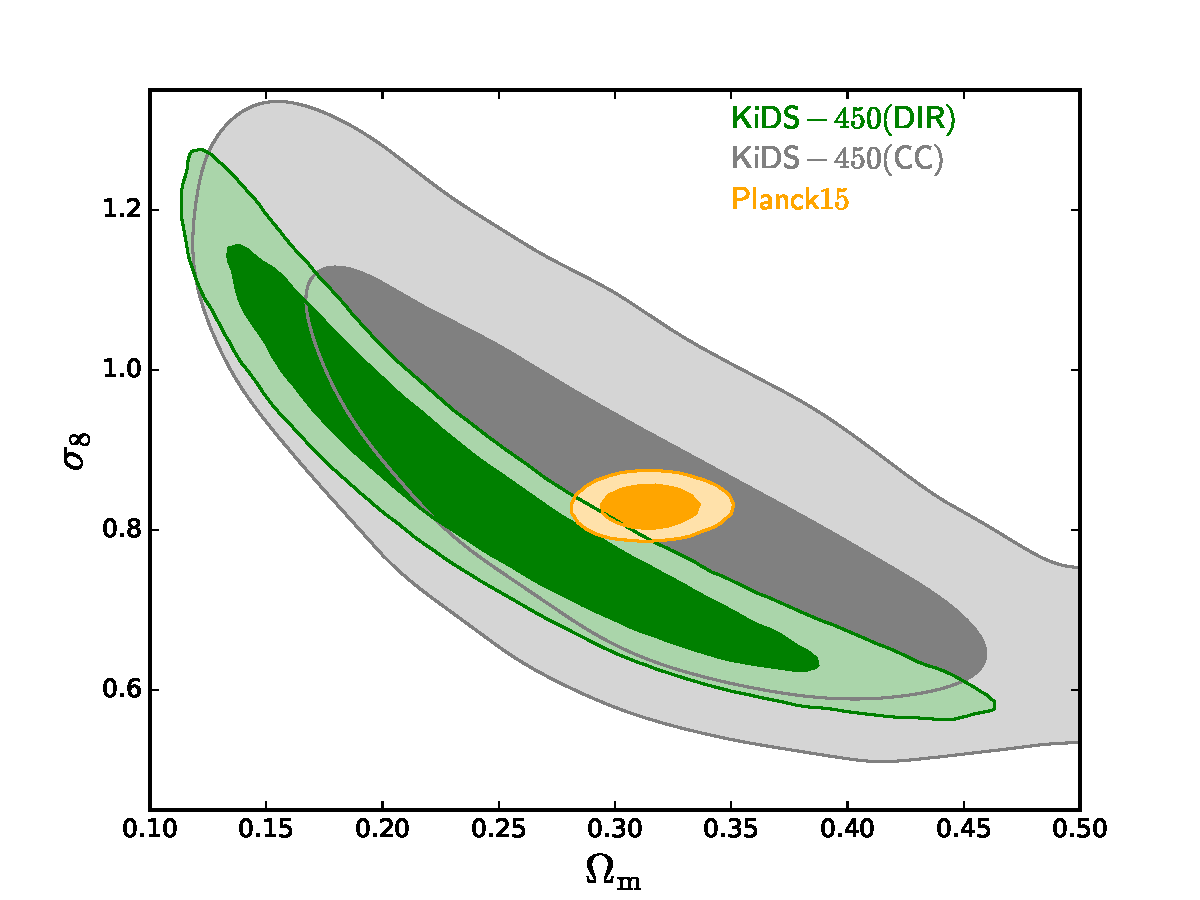
\includegraphics[width=\textwidth]{banana_DIR_vs_CC_vs_Planck.pdf}
  \end{minipage}\hfill
  \begin{minipage}[c]{0.35\textwidth}
    \caption*{Fig.~1: Cosmology constraints from KiDS-450 using the different photometric redshift calibration strategies. Note the tension between Planck and the most precise (DIR) calibration. The aim of this proposal is to reduce the CC errors by a factor of $\sqrt{10}$ to bring them in line with the DIR calibration accuracy, and to prepare for the analysis of the next, twice as extensive, KiDS lensing data.}
  \end{minipage}
\end{figure}
\end{document}
